\chapter{Mengenal Kecerdasan Buatan dan Scikit-Learn}
Buku umum yang digunakan adalah \cite{russell2016artificial} dan  
untuk sebelum UTS menggunakan buku \textit{Python Artificial Intelligence Projects for Beginners}\cite{eckroth2018python}.
Dengan praktek menggunakan python 3 dan editor anaconda dan library python scikit-learn.
Tujuan pembelajaran pada pertemuan pertama antara lain:
\begin{enumerate}
\item
Mengerti definisi kecerdasan buatan, sejarah kecerdasan buatan, perkembangan dan penggunaan di perusahaan
\item
Memahami cara instalasi dan pemakaian sci-kit learn
\item
Memahami cara penggunaan variabel explorer di spyder
\end{enumerate}
Tugas dengan cara dikumpulkan dengan pull request ke github dengan menggunakan latex pada repo yang dibuat oleh asisten riset.

\section{Teori}
Praktek teori penunjang yang dikerjakan :
\begin{enumerate}
\item
Buat Resume Definisi, Sejarah dan perkembangan Kecerdasan Buatan, dengan bahasa yang mudah dipahami dan dimengerti. Buatan sendiri bebas plagiat[hari ke 1](10)
\item
Buat Resume mengenai definisi supervised learning, klasifikasi, regresi dan unsupervised learning. Data set, training set dan testing set.[hari ke 1](10)
\end{enumerate}

\section{Instalasi}
Membuka https://scikit-learn.org/stable/tutorial/basic/tutorial.html. Dengan menggunakan bahasa yang mudah dimengerti dan bebas plagiat. 
Dan wajib skrinsut dari komputer sendiri.
\begin{enumerate}
\item
Instalasi library scikit dari anaconda, mencoba kompilasi dan uji coba ambil contoh kode dan lihat variabel explorer[hari ke 1](10)
\item
Mencoba Loading an example dataset, menjelaskan maksud dari tulisan tersebut dan mengartikan per baris[hari ke 1](10)
\item
Mencoba Learning and predicting, menjelaskan maksud dari tulisan tersebut dan mengartikan per baris[hari ke 2](10)
\item
mencoba Model persistence, menjelaskan maksud dari tulisan tersebut dan mengartikan per baris[hari ke 2](10)
\item 
Mencoba Conventions, menjelaskan maksud dari tulisan tersebut dan mengartikan per baris[hari ke 2](10)
\end{enumerate}


\section{Penanganan Error}
Dari percobaan yang dilakukan di atas, apabila mendapatkan error maka:

\begin{enumerate}
	\item
	skrinsut error[hari ke 2](10)
	\item
Tuliskan kode eror dan jenis errornya [hari ke 2](10)
	\item
Solusi pemecahan masalah error tersebut[hari ke 2](10)

\end{enumerate}


\section{Fathi Rabbani / 1164074}
\subsection{Teori}
\begin{enumerate}
\item
Sejarah dan Perkembangan Kecerdasan Buatan
\subitem
Sejarah dari sebuah Artificial Intelligence atau dalam Bahasa indonesianya diterjemahkan sebagai Kecerdasan Buatan adalah sebuah usaha untuk dapat memodelkan sebuah mesin agar dapat berfikir dan menirukan tingkah laku dan cara berfikir manusia, ada beberapa jenis dari kecerdasan buatan, yaitu :

\begin{itemize}
\item
Symbol Manipulating AI
\item
Nueral AI
\item
Neural Network
\end{itemize}
\subitem
Peneliti yang selalu disebutkan sebagai Bapak AI adalah Jhon McCharty  merupakan seorang dosen yang mengenalkan Kecerdasan Buatan kepada 2 lembaga penelitian hebat, yaitu Stanford Artificial Intelligence Laboratory dan MIT Artificial Intelligence Laboratory.
\subitem
Sedangkan perkembangan kecerdasan buatan saat ini sudah mencapai tahap dimana manusia mulai membuat sebuah robot yang dapat menirukan hampir 90 persen dari keseharian mereka, mulai dari bidang kesehatan, koki, pabrik, kantoran, hingga sebuah robot yang bertugas sebagai seorang pelayan di sebuah restoran. Dan dubai sebagai pengguna mobil tanpa pengemudi yang menerapkan AI dengan menggunakan data wilayah serta jarak kendaraan dengan pingir jalan.
\item
Definisi Supervised, Unsupervised Learning, Klasifikasi, Regresi serta Data, Training, Testing Set
\begin{itemize}
\item
Supervised learning merupakan sebuah pendekatan AI dengan latihan yang sudah dilakukan dengan sebuah data yang lengkap, dan memiliki variable yang dapat digunakan sebagai target sehingga dapat menujukan data agar menjadi kelompok dari sebuah data menjadi kelompok data yang baru.
\item
Unsupervised learning merupakan sebuah pendekatan AI tanpa menggunakan data yang lengkap dan ter-variable sehingga harus dilakukan pengelompokkan agar data tersebut dapat digunakan.
\item
Klasifikasi merupakan sebuah pengelompokkan suatu objek ke dalam kategori tertentu.
\item
Regresi merupakan pendekatan model matematika untuk mendeskripsikan hubungan dari beberapa variabel independen dengan variable dependen.
\item
Data Set, meupakan sebuah objek yang merepresentasikan data dan hubungannya di memory. 
\item
Training Set, subset untuk melatih model.
\item
Testing Set, subset untuk menguji model yang sudah dilatih.
\end{itemize}


\subsection{Praktikum}
\item
Instalasi Library Scikit dari Anaconda

\subitem
Pertama Download terlebih dahulu anaconda-nya di https://www.anaconda.com/distribution/ pilih Operating Sistem yang kalian gunakan. lalu setelah download Install dengan proses berikut :
\begin{itemize}
\item
Proses Instalasi Anaconda pada gambar \ref{proses2} hingga proses \ref{proses9}.
\item
Proses Instalasi Scikit-Learn dengan menggunakan Conda pada gambar \ref{proses10} hingga gambar \ref{proses12}.
\item
contoh dari Variable Explorer yang digunakan ada pada gambar \ref{proses14}.
\end{itemize}
\begin{figure}[ht]
\centerline{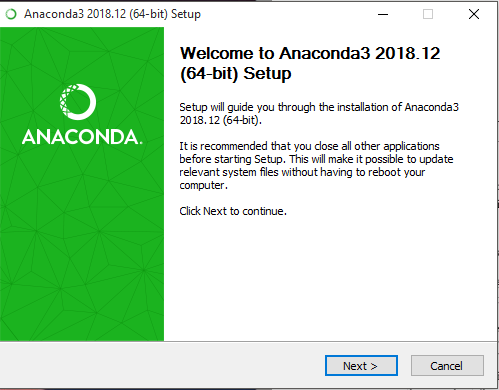
\includegraphics[width=1\textwidth]{figures/fathi/2.PNG}}
\caption{setelah membuka data instalasi klik next}
\label{proses2}

\centerline{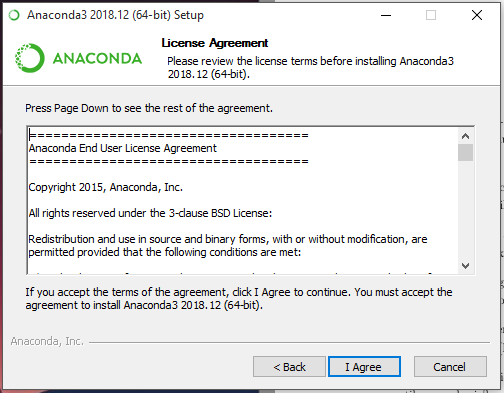
\includegraphics[width=1\textwidth]{figures/fathi/3.PNG}}
\caption{pilih i agree}
\label{proses3}
\end{figure}
\begin{figure}
\centerline{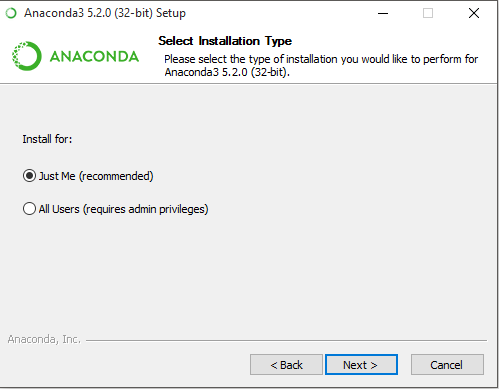
\includegraphics[width=1\textwidth]{figures/fathi/4.PNG}}
\caption{pilih instalasi Just Me}
\label{proses4}

\centerline{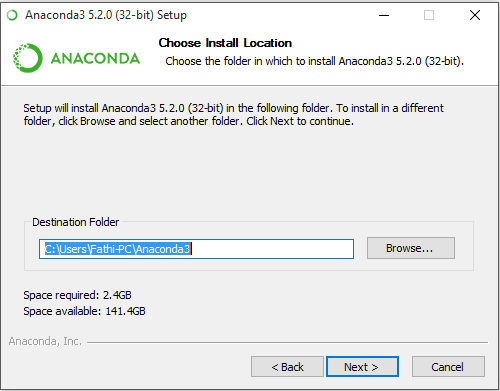
\includegraphics[width=1\textwidth]{figures/fathi/5.PNG}}
\caption{langsung saja next}
\label{proses5}
\end{figure}
\begin{figure}
\centerline{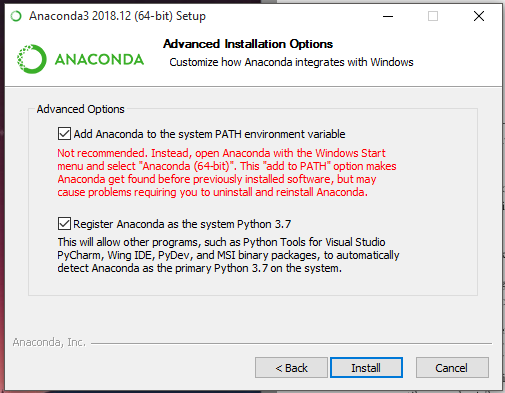
\includegraphics[width=1\textwidth]{figures/fathi/6.PNG}}
\caption{cek kedua pilihan tersebut}
\label{proses6}

\centerline{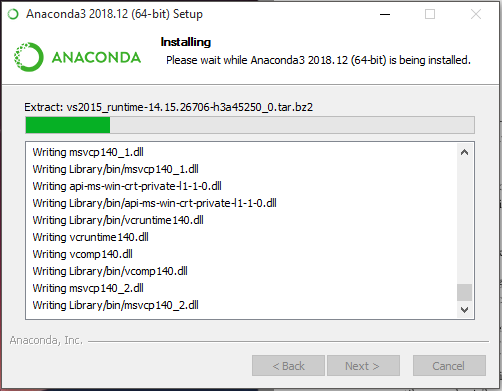
\includegraphics[width=1\textwidth]{figures/fathi/7.PNG}}
\caption{proses Instalasi}
\label{proses7}
\end{figure}
\begin{figure}
\centerline{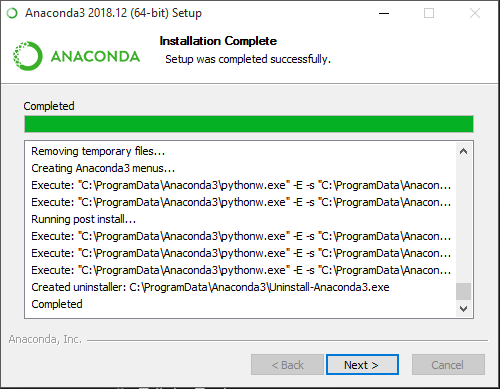
\includegraphics[width=1\textwidth]{figures/fathi/8.PNG}}
\caption{klik next}
\label{proses8}

\centerline{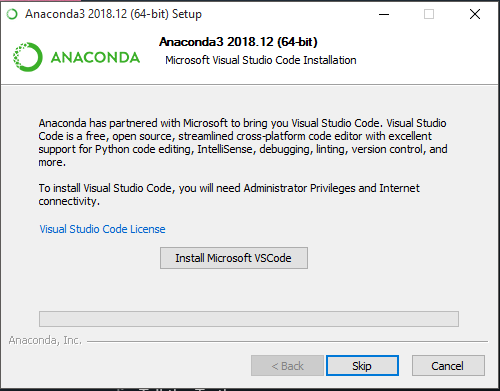
\includegraphics[width=1\textwidth]{figures/fathi/9.PNG}}
\caption{selesai instalasi anaconda}
\label{proses9}
\end{figure}
\begin{figure}
\centerline{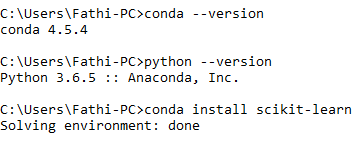
\includegraphics[width=1\textwidth]{figures/fathi/10.PNG}}
\caption{Instalasi SCIKIT dengan menggunakan anaconda}
\label{proses10}

\centerline{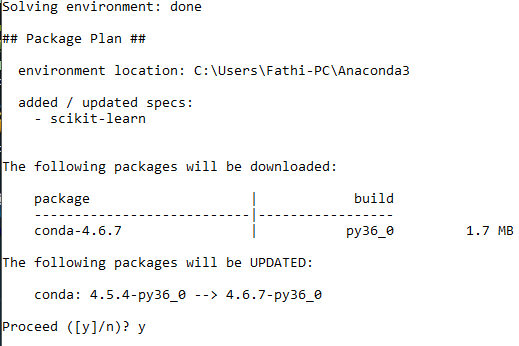
\includegraphics[width=1\textwidth]{figures/fathi/11.PNG}}
\caption{Konfirmasi Instalasi}
\label{proses11}
\end{figure}
\begin{figure}
\centerline{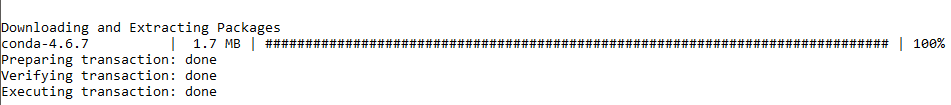
\includegraphics[width=1\textwidth]{figures/fathi/12.PNG}}
\caption{hasil dari instalasi SCIKIT}
\label{proses12}
\centerline{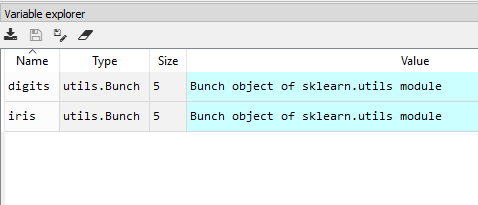
\includegraphics[width=1\textwidth]{figures/fathi/14.PNG}}
\caption{data variable explorer}
\label{proses14}
\end{figure}

\item
Load Example Dataset dan Menjeleaskan kegunakan barisan Code
\subitem
berikut ini adalah contoh dataset yang digunakan untuk melakukan compile ada pada gambar \ref{proses16} dan hasilnya ada pada gambar \ref{proses15}.

\begin{figure}
\centerline{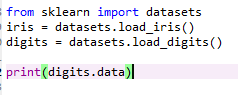
\includegraphics[width=1\textwidth]{figures/fathi/16.PNG}}
\caption{code example dataset yang digunakan}
\label{proses16}

\centerline{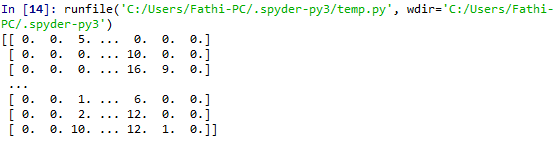
\includegraphics[width=1\textwidth]{figures/fathi/15.PNG}}
\caption{data hasil dari code example dataset yang digunakan}
\label{proses15}
\end{figure}
\begin{itemize}
\item
dari code yang dicoba diketahui bahwa data set yang digunakan adalah data yang diambil dari SKLEARN yang ada pada gambar \ref{proses16}.
\end{itemize}
\end{enumerate}
